\documentclass[11pt,letterpaper]{article}
\usepackage[utf8]{inputenc}

%----- Configuración del estilo del documento------%
\usepackage{epsfig,graphicx}
\usepackage[left=2cm,right=2cm,top=1.8cm,bottom=2.3cm]{geometry}
\usepackage{fancyhdr}
\usepackage{lastpage}

\usepackage{xcolor}
\usepackage{soul}
\newcommand{\mathcolorbox}[2]{\colorbox{#1}{$\displaystyle #2$}}

%Color bibi
\definecolor{bibi}{RGB}{0,103,148}
% Otros colores

%------ Paquetes matemáticos básicos --------%
\usepackage{amsmath}
\usepackage{amssymb}
\usepackage{amsthm}

%------ Paquetes para codigo --------%
\usepackage{verbatim}
\usepackage{listings}
\lstset{language=Haskell, basicstyle=\ttfamily, keywordstyle=\color{blue}, commentstyle=\color{gray}, stringstyle=\color{green}}

\usepackage{tikz}

%------ Paquete para posicionamiento de figuras --------%
\usepackage{float}

%------ Paquete para bibliografia --------%
\usepackage[backend=biber,style=numeric]{biblatex}
\addbibresource{src/bibliografia.bib} % 


\begin{document}

%------ Encabezado -------- %
\begin{center}
    \begin{minipage}{3cm}
    	\begin{center}
    		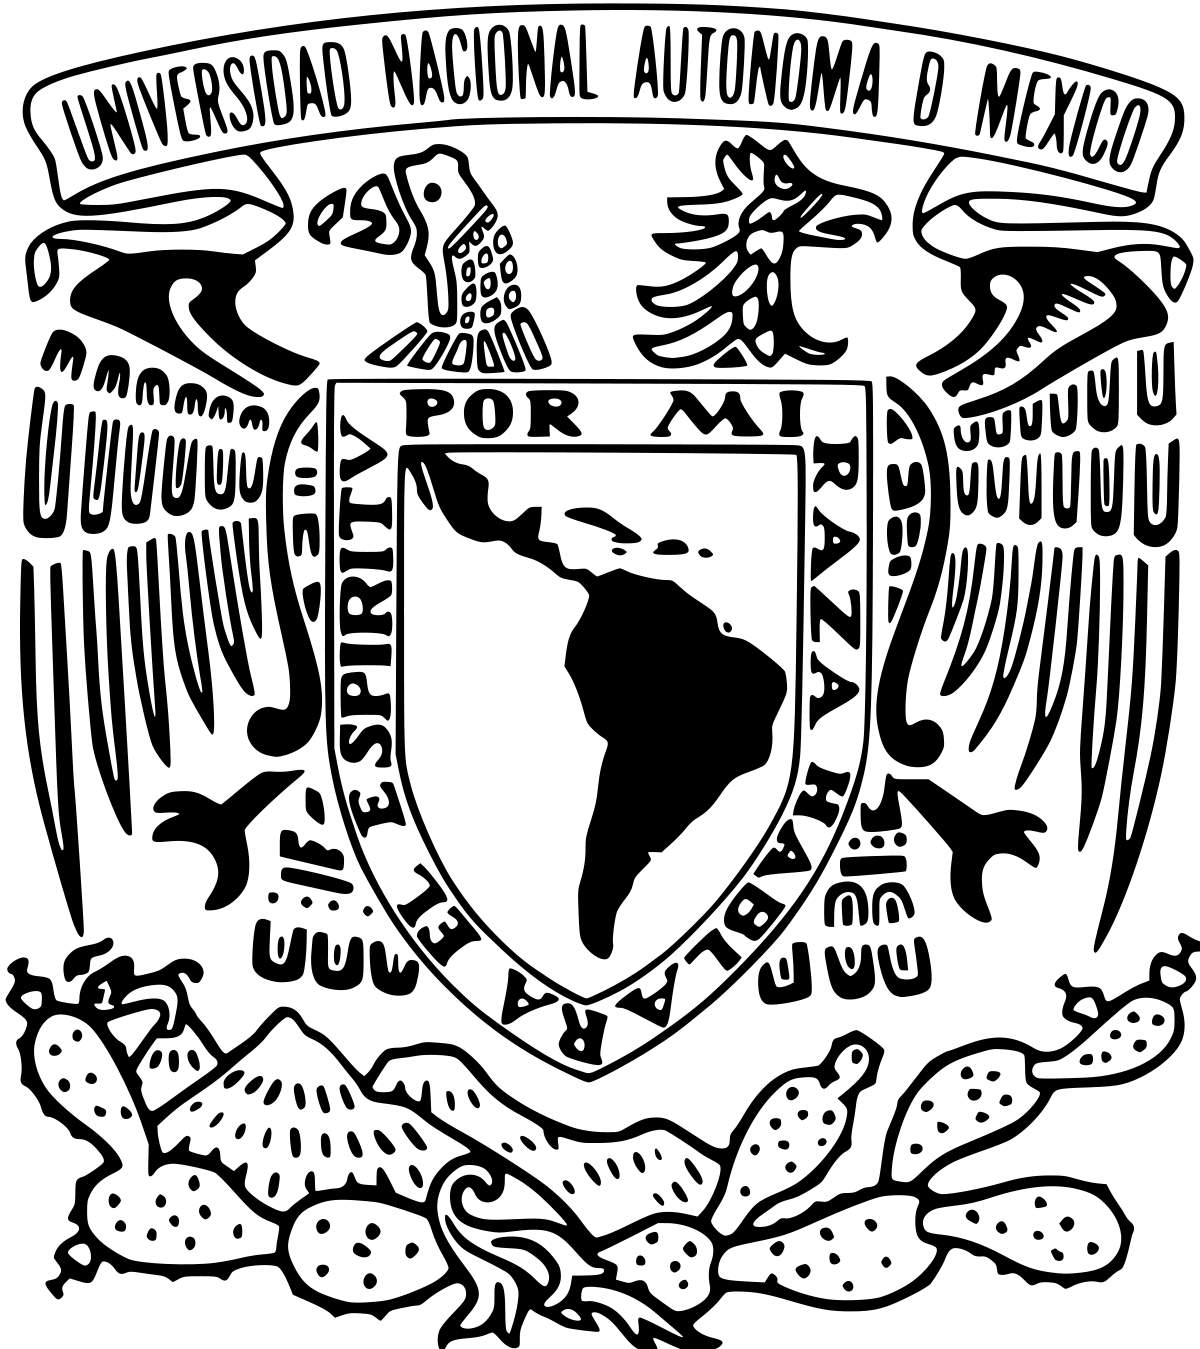
\includegraphics[height=3.2cm]{src/Img/Logo_UNAM.png}
    	\end{center}
    \end{minipage}\hfill
    \begin{minipage}{10cm}
    	\begin{center}
    	\textbf{\large Universidad Nacional Autónoma de México}\\[0.1cm]
        \textbf{Facultad de Ciencias}\\[0.1cm]
        \textbf{Sistemas Operativos  $|$ 7006}\\[0.1cm]
        Práctica 01 : $|$ Maquinas virtuales \\[0.1cm]
        Sosa Romo Juan Mario $|$ 320051926 \\[0.1cm]
        16/03/24
    	\end{center}
    \end{minipage}\hfill
    \begin{minipage}{3cm}
    	\begin{center}
    		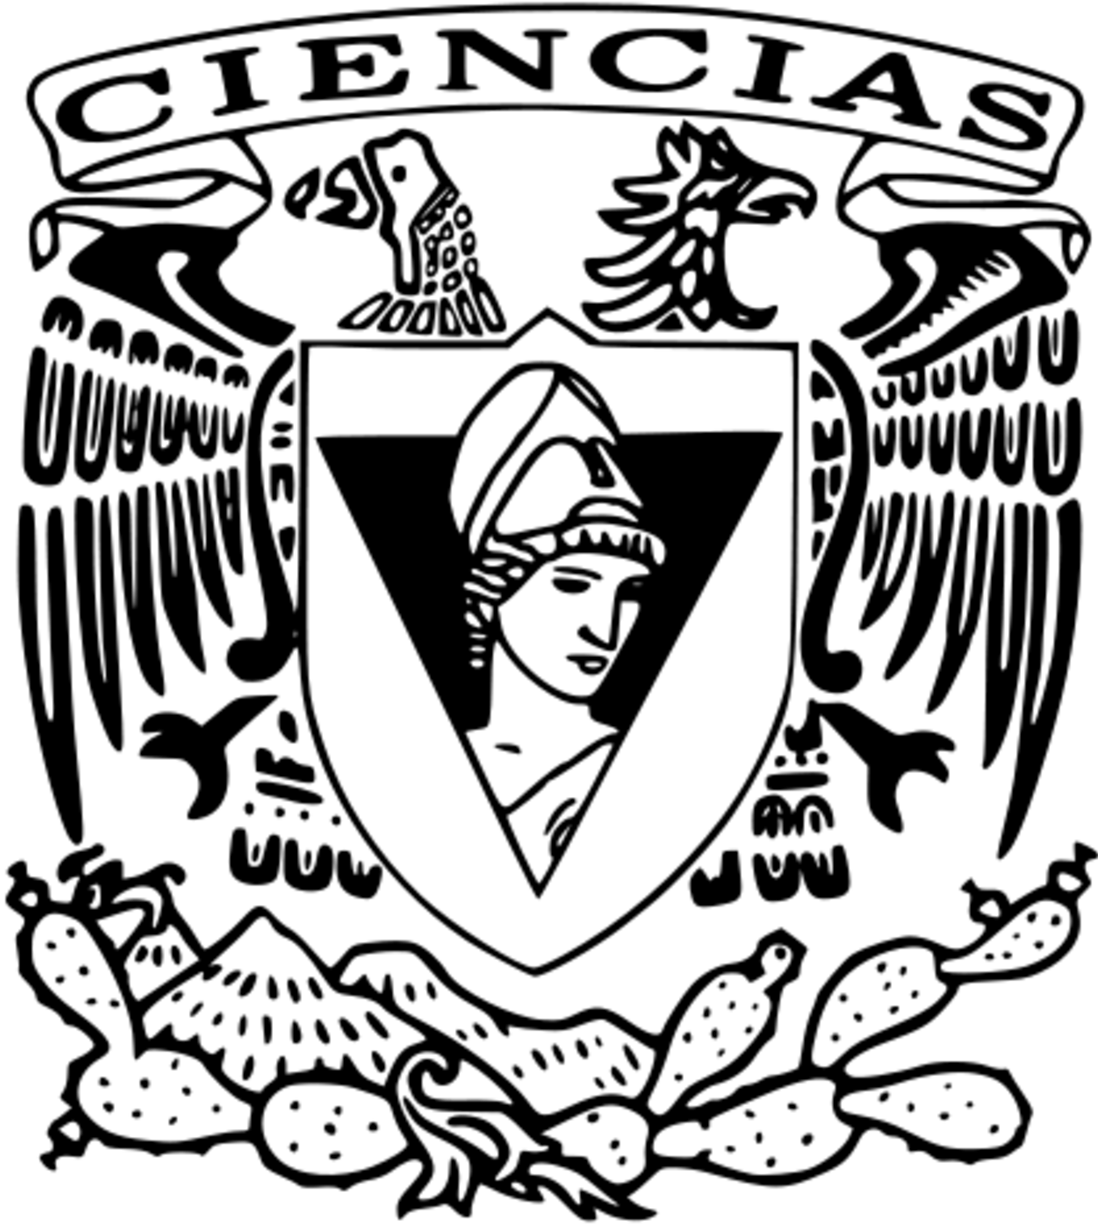
\includegraphics[height=3.2cm]{src/Img/Logo_FC.png}
    	\end{center}
    \end{minipage}
\end{center}


\rule{16.9cm}{0.1mm}
\vspace{0.3cm}

\vspace{0.3cm}
%------ Preguntas -------- %
\begin{enumerate}
    \item \textbf{Crea una variable llamada 'mio' con tu nombre, deberás hacer 'echo' a la variable y mostrar tu nombre. Toma captura de pantalla del proceso y del resultado de la llamada al programa 'echo'.}  \vspace{0.3cm}

\begin{figure}[H]
    \centering
    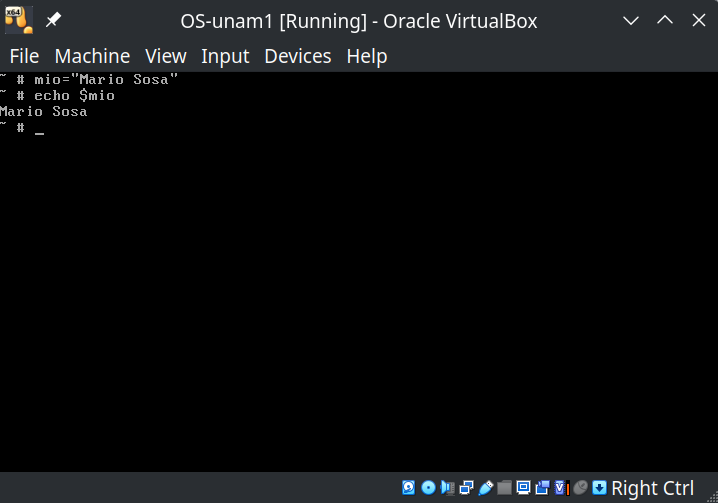
\includegraphics[height=8cm]{src/Img/1.png}
    \caption{echo de la variable 'mio'.}
    \label{fig:echoMio}
\end{figure}


\item \textbf{Investiga y da una breve explicación sobre para qué sirve el comando 'uname'.}  \vspace{0.3cm}

Primero que nada el nombre del comando literalmente sale del acrónimo 'UNIX name', por su nombre entonces sabemos que es una herramienta que nos permite encontrar información util sobre el sistema operativo y el kernel. \vspace{.2cm}

Por lo que investigue, el comando utiliza una estructura de datos en el sistema que se llama 'utsname', ahi tiene literalmente la información que queremos recuperar. \vspace{.2cm}

Ademas, el comando tiene varias opciones utiles por si quieres cosas especificas, como por ejemplo '-a' que te da toda la información que tiene el comando, o '-s' que te da el nombre del kernel. \vspace{.2cm} \cite{gnu_uname}

\item \textbf{¿Cómo se llama el kernel del sistema operativo que estamos usando?}  \vspace{0.3cm}

Como mencione en el punto anterior, basta con utilizar el comando 'uname -s' para obtener el nombre del Kernel que en este caso se llama igual que el nombre y numero del curso "Sistemas Operativos 7006" \vspace{.2cm}

\begin{figure}[H]
    \centering
    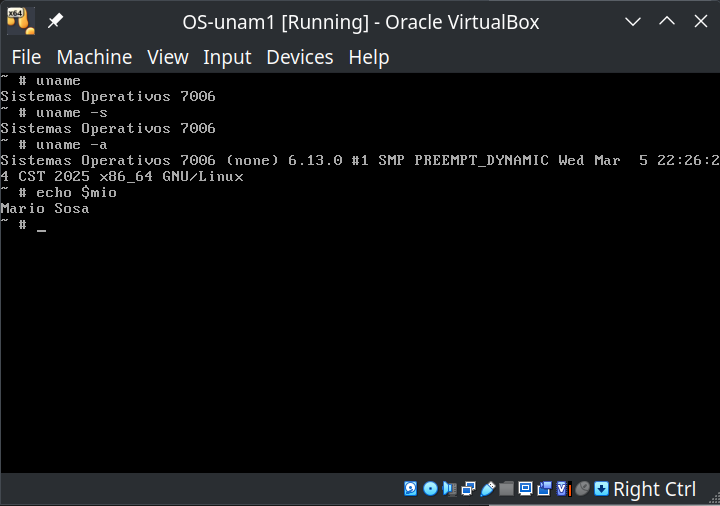
\includegraphics[height=8cm]{src/Img/2.png}
    \caption{Todos los comandos anteriores}
    \label{fig:allcmd}
\end{figure}

\item \textbf{Investiga cómo tomar el compilado de un programa cualquiera (en el lenguaje que sea) y dónde tenemos que guardarlo para poder usarlo como comando.}  \vspace{0.3cm}

Asumiendo que ya tienes el ejecutable, digamos que se llama 'programa', debemos poner el archivo en uno de los directorios listados en la variable de entorno 'PATH', ejemplos de estas carpetas son por ejemplo:\vspace{.2cm}

\begin{itemize}
    \item /bin
    \item /usr/bin
    \item /usr/local/bin
\end{itemize} \vspace{.2cm}

Entonces por ejemplo podemos mover el archivo a '/usr/local/bin' y ya podremos ejecutar el programa desde cualquier lugar, aunque es posible que ocupes permisos para poder mover el archivo ahi. Despues es tan simple como utilizar el nombre del archivo para ejecutarlo. \cite{compilado2023} \vspace{.2cm} 


\textbf{Problemas y notas:}  \vspace{0.3cm}

Tuve nada mas 2 problemitas, el primero fue a la hora de crear el disco porque no le gusto donde lo guarde (tambien es que lo movi y no te deja re direccionar el apuntador) y el segundo fue todo lo relacionado a IO en la VM, como siempre, obviamente cualquier uso del mouse no sirve y el teclado tiene otra distribución de teclas. \vspace{.2cm}



\end{enumerate}

\printbibliography

\end{document}